\documentclass[12pt, a4paper]{article}
\usepackage{ctex} % 中文的宏包
\usepackage{indentfirst}
\usepackage{graphicx} % 插入圖片的宏包
\usepackage{float} % 設置圖片浮動位置的宏包
\usepackage{subfigure} % 插入多圖時用子圖顯示宏包
\usepackage{listings} % 代碼塊宏包
\usepackage{color} % 代碼高亮
\usepackage[colorlinks,linkcolor=blue]{hyperref} % URL 包
\usepackage[pdf]{graphviz}

\definecolor{dkgreen}{rgb}{0,0.6,0}
\definecolor{gray}{rgb}{0.5,0.5,0.5}
\definecolor{mauve}{rgb}{0.58,0,0.82}

\lstset{ %
    %language=Octave,                % the language of the code
    basicstyle=\scriptsize\Hack,           % the size of the fonts that are used for the code
    numbers=none,                   % where to put the line-numbers
    numberstyle=\tiny\color{gray},  % the style that is used for the line-numbers
    stepnumber=2,                   % the step between two line-numbers. If it's 1, each line 
                                    % will be numbered
    numbersep=3pt,                  % how far the line-numbers are from the code
    backgroundcolor=\color{white},      % choose the background color. You must add \usepackage{color}
    showspaces=false,               % show spaces adding particular underscores
    showstringspaces=false,         % underline spaces within strings
    showtabs=false,                 % show tabs within strings adding particular underscores
    frame=single,                   % adds a frame around the code
    rulecolor=\color{black},        % if not set, the frame-color may be changed on line-breaks within not-black text (e.g. commens (green here))
    tabsize=2,                      % sets default tabsize to 2 spaces
    captionpos=b,                   % sets the caption-position to bottom
    breaklines=true,                % sets automatic line breaking
    breakatwhitespace=false,        % sets if automatic breaks should only happen at whitespace
    title=\lstname,                   % show the filename of files included with \lstinputlisting;
                                    % also try caption instead of title
    keywordstyle=\color{blue},          % keyword style
    commentstyle=\color{dkgreen},       % comment style
    stringstyle=\color{mauve},         % string literal style
    escapeinside={\%*}{*},            % if you want to add LaTeX within your code
    morekeywords={*,...}               % if you want to add more keywords to the set
}
\setCJKmainfont{Noto Serif CJK TC} % 主要字體 Noto Serif
\newfontfamily\Hack{Hack} % 代碼字體
\author{軟件 1804 8209180438 黃柏曛}
\date{\today}
\title{編譯原理 教材第 36 頁 6 7 8 9 題}
\begin{document}
\maketitle
\section{P36 第 6 題}
    \subsection{$G_{6}$ 的語法 $L(G_{6})$ 是什麼?}
    
    $L(G_{6})$ 是 $0\sim9$ 的字符串。

    \subsection{給出句子 0127、34 和 567 的最左推導和最右推導。}

    {最左推導:}

    {\footnotesize $N \Rightarrow ND \Rightarrow NDD \Rightarrow NDDD \Rightarrow DDDD \Rightarrow 0DDD \Rightarrow 01DD \Rightarrow 012D \Rightarrow 0127$}

    {\footnotesize $N \Rightarrow ND \Rightarrow DD \Rightarrow 3D \Rightarrow 34$}

    {\footnotesize $N \Rightarrow ND \Rightarrow NDD \Rightarrow DDD \Rightarrow 5DD \Rightarrow 56D \Rightarrow 568$ }\\

    {最右推導:}
    
    {\footnotesize $N \Rightarrow ND \Rightarrow N7 \Rightarrow N27 \Rightarrow ND27 \Rightarrow N127 \Rightarrow D127 \Rightarrow 0127$ }
    
    {\footnotesize $N \Rightarrow ND \Rightarrow N4 \Rightarrow D4 \Rightarrow 34$}
    
    {\footnotesize $N \Rightarrow ND \Rightarrow N8 \Rightarrow ND8 \Rightarrow N68 \Rightarrow D68 \Rightarrow 568$}

\section{P36 第 7 題}
    \subsection{寫一個文法,使其語言是奇數集,且每個奇數不以 0 開頭。}

    {$G(S)$}

    {$O \rightarrow 1 \mid 3 \mid 5 \mid 7 \mid 9$}

    {$N \rightarrow 2 \mid 4 \mid 6 \mid 8 \mid O$}

    {$D \rightarrow 0 \mid N$}

    {$S \rightarrow O \mid AO$}

    {$A \rightarrow AD \mid N$}

\section{P36 第 8 題}
    \subsection{給出 i + i * i、i * (i + i) 的最左推導與最右推導}

    {文法:}

    {$E \rightarrow T \mid E + T \mid E - T$}

    {$T \rightarrow F \mid T * F \mid T / F$}

    {$F \rightarrow (E) \mid i$}\\

    {最左推導:}

    {$E \Rightarrow E + T \Rightarrow T + T \Rightarrow F + T \Rightarrow i + T \Rightarrow i + T * F \Rightarrow i + F * F \Rightarrow i + i * F \Rightarrow i + i * i$}

    {$E \Rightarrow T \Rightarrow T * F \Rightarrow F * F \Rightarrow i * F \Rightarrow i * (E) \Rightarrow i * (E + T) \Rightarrow i * (T + T) \Rightarrow i * (F + T) \Rightarrow i * (i + T) \Rightarrow i * (i + F) \Rightarrow i * (i + i)$}\\

    {最右推導:}

    {$E \Rightarrow E + T \Rightarrow E + T * F \Rightarrow E + T * i \Rightarrow E + i * i \Rightarrow T + i * i \Rightarrow F + i * i \Rightarrow i + i * i$}

    {$E \Rightarrow T \Rightarrow F * T \Rightarrow F * F \Rightarrow F * E \Rightarrow F * (E + T) \Rightarrow F * (E + F) \Rightarrow F * (E + i) \Rightarrow F * (T + i) \Rightarrow F * (F + i) \Rightarrow F * (i + i) \Rightarrow i * (i + i)$}

    \subsection{語法樹}

    \begin{figure}[H]
        \centering  %图片全局居中
        \subfigure[i + i + i]{
        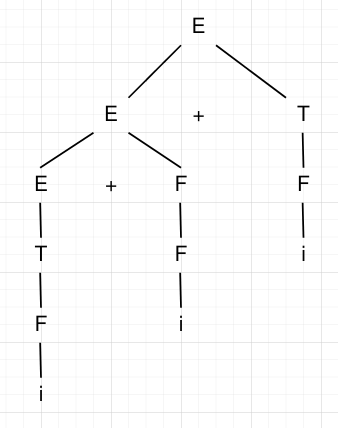
\includegraphics[width=0.45\textwidth]{i+i+i.png}}
        \subfigure[i - i - i]{
        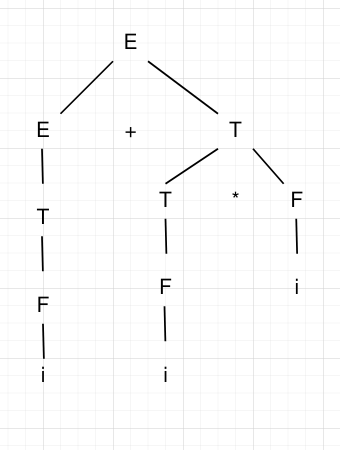
\includegraphics[width=0.45\textwidth]{i-i-i.png}}
        \subfigure[i + i * i]{
        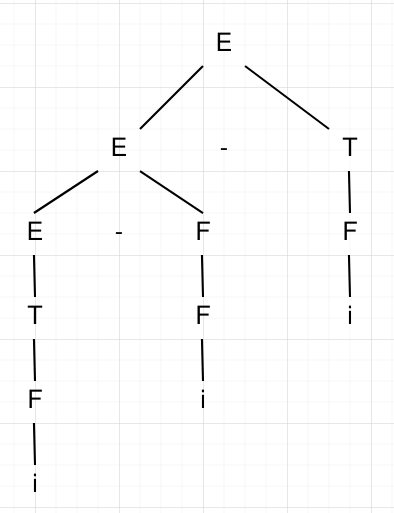
\includegraphics[width=0.45\textwidth]{i+i*i.png}}
    \end{figure}

\section{P36 第 9 題}
    \subsection{證明文法 $S \rightarrow iSeS \mid iS \mid i$ 是二義的。}

    {iiiei 句子中有兩個語法樹:}\\

    {$S \Rightarrow iSeS \Rightarrow iSei \Rightarrow iiSei \Rightarrow iiiei$}

    {$S \Rightarrow iS \Rightarrow iiSeS \Rightarrow iiSei \Rightarrow iiiei$}\\

    {故可以證明 $S \rightarrow iSeS \mid iS \mid i$ 是二義的。}

\end{document}